\documentclass[12pt]{report}
\usepackage{polski}
\usepackage[utf8]{inputenc}
\usepackage{indentfirst}
\usepackage[margin=1in]{geometry}
\usepackage[nottoc]{tocbibind}
\usepackage{graphicx}
\usepackage{chngcntr}
\setlength{\parskip}{1ex plus 0.5ex minus 0.2ex}
\counterwithout{figure}{chapter}
\linespread{1.5}
\author{Grzegorz Kastelik}
\title{Praca inżynierska}
\frenchspacing

\begin{document}
    \thispagestyle{empty}

\begin{center}

    AKADEMIA TECHNICZNO-HUMANISTYCZNA

    W BIELSKU - BIAŁEJ
    \vspace{0.5cm}
    
    WYDZIAŁ BUDOWY MASZYN I INFORMATYKI
    \vspace{0.6cm}

    \textbf{ {\Large PRACA DYPLOMOWA} \\
    INŻYNIERSKA nr .......... \\
    Grzegorz Kastelik \\}
    \vspace{0.5cm}
    {\small
    Nr albumu: 051414 \\
    Kierunek: Informatyka \\
    Specjalność: Inżynieria Oprogramowania i Systemy Informatyczne \\}
    \vspace{0.5cm}

    Temat pracy: Platforma umożliwiająca generowanie dokumentów i umów na podstawie interaktywnych szablonów 



    {\small 
        \begin{flushleft}
            Zakres pracy:\\
            1. Analiza problemu i określenie wymagań funkcjonalnych i pozafunkcjonalnych  \\
            2. Wybór technologii i narzędzi realizacji \\
            3. Opracowanie systemu tworzenia i generowania umów \\
            4. Utworzenie platformy internetowej implementującej opracowany system \\
            5. Konfigurowanie komponentów użytych w platformie \\
            6. Edycja pisemna pracy \\
            \vspace{0.5cm}
            Kategoria rodzaju pracy: ..........
        \end{flushleft}
    
        \textbf{Katedra Informatyki i Automatyki / Zakład Informatyki}
    
        \begin{flushleft}
            Promotor: \textbf{dr. Łukasz Więcław}
        \end{flushleft}
    
        \begin{flushright}
            ................................. \\
            Podpis i pieczątka \\
            Kierownika Katedry \\
        \end{flushright}
        
        Bielsko-Biała, rok akademicki ..........
    }

\end{center}

\newpage
    \tableofcontents
    \chapter*{Wstęp}
    \addcontentsline{toc}{chapter}{Wstęp}
        Rozwój technologii jaki obserwujemy na przestrzeni ostatnich lat, znacząco pozwala nam na stwierdzenie, iż pełna cyfryzacja usług to kierunek dla każdej nowoczesnej firmy, instytucji, czy też państw. Społeczeństwo, szczególnie młodsze, bardzo szybko adaptuje nowoczesne rozwiązania w dostarczaniu usług. Można powiedzieć, że kierunek cyfryzacji jest wręcz wymuszony, aby dana firma mogła przetrwać i sprawnie funkcjonować na runku. 

Ludzie nauczyli się, iż taka forma świadczenia usług niesie za sobą szereg korzyści. Jest często tańsza, gdyż nie wymusza posiadania dodatkowych pracowników do zarządzania. Szybsza i wygodniejsza, gdyż pozwala na skorzystanie bez wychodzenia z domu. Może z niej skorzystać wiele osób w jednym czasie. Nie trzeba do tego stać w kolejkach znacząco przyczynia się do oszczędzania czasu jaki trzeba poświęcić. 

Przedsiębiorstwa są nie tylko zmuszone do cyfryzacji, ale jednocześnie zachęcone. Pomimo kosztów początkowych mają one szanse na efektywne skalowanie swoich usług i dostarczenie ich większej ilości użytkowników niż dotychczas. 

Taka sytuacja nie ominęła również prawników. Zmotywowani automatyzacją są gotowi i chętni część swojej wiedzy przenieść w świat wirtualny. Duża część pracy prawniczej jest schematyczna, szczególnie tworzenie umów dla klientów. Wykorzystując ten fakt, można z łatwością znaleźć zastosowania dla cyfryzacji w owym środowisku. Dzięki takiemu zabiegowi otwierają się na wielu nowych klientów, całkowicie globalnie, ponieważ jedyne co potrzebuje klient to połączenie z Internetem i przeglądarka. Usługi takie mogą świadczyć dużo taniej, gdyż nie skupiają swojego czasu na schematycznych działań i mogą skupić się na najważniejszych aspektach swojej pracy. 

Platforma do tworzenia umów ma więc bardzo praktyczne zastosowanie i jest dla prawników niezbędna, jeśli chcą wejść w świat usług wirtualnych. Jest ona stworzona, aby maksymalnie ułatwić i zautomatyzować ich pracę bez konieczności pomocy z zewnątrz, oraz specjalistycznej wiedzy z zakresu programowania i technologii internetowych. 

    \chapter*{Cel i zakres pracy}
    \addcontentsline{toc}{chapter}{Cel i zakres pracy}
        \textit{\textbf{Celem pracy było zaprojektowanie systemu umożliwiającego tworzenia umów prawniczych zaimplementowanego jako platforma Internetowa.}}

\vspace{1cm}

System tworzenia umów w swojej podstawowej formie ma za zadanie dostarczyć platformę Internetową oraz API umożliwiającej pełną obsługę wyłączając z tego proce budowy szablony umowy za pomocą bloków. Jego zadaniem jest umożliwić wszystkie działania związane z platformą, szczególnie dostarczać wszelkie informacje potrzebne do dynamicznego generatora szablonów tworzonych jako osobna część w platformie ze względu na poziom skomplikowania i potrzebę dopracowania elementów pod finalnych użytkowników.

W zakres pracy wchodzi więc utworzenie API które umozliwia pełne zarządzanie całym system oraz platformę która będzie mogła korzystać z API w celu wykonywania akcji związanych z tworzeniem umów, wypełnianiem, oraz zarządzaniem całym systemem.

    \chapter{Specyfikacja}
        \section{Umowy}
            Na początek warto przytoczyć podstawową definicję pojęcia umowy, jest to:

\begin{quote}
    „Wzajemne uzgodnienie dwóch lub więcej stron mająca na celu obopólne dobro oraz określająca wzajemne obowiązki oraz prawa stron.” \cite{enc-zarzadzania}
\end{quote}

Umowy zawierać można na wiele sposobów, każdy kraj dodaje swoje obostrzenia jednak w większości możliwe jest utworzenie umowy w wersji pisemnej z podpisem i egzemplarzem dla każdej ze stron.  

Każda umowa to odrębna sytuacja jednak wiele z nich podchodzi pod schemat, dzięki któremu możemy zautomatyzować czynności. Bazując na tym platforma umożliwia tworzenie takich oto schematów, aby mogły być w automatyczny sposób dostarczane do wielu klientów i przez wielu na raz wypełniane. 

Wypełnienie wiąże się z procesem z góry określonym przez który musi przejść użytkownik, aby uzyskać umową, którą będzie musiał jedynie wypełnić. Proces ten w większości przypadków to zebranie takich danych jakie potrzeba, aby idealnie przygotować umowę pod daną osobę. 

Umowy występują jednak pod różnymi poziomami skomplikowania. Część to proste jednostronne umowy z prostym systemem. Kolejne to umowy kilkunastu stronnicowe precyzyjnie określające wszystkie możliwe akcje. Wiąże się to z dużą ilością danych jakie trzeba zebrać, przetworzyć i w zgodzie z nimi zbudować umowę końcową.

        \section{Platforma internetowa}
            Platforma internetowa to dzisiaj jeden z najczęściej spotykanych typów aplikacji. Jej wszechstronność i dostępność znacząco odbiegają od innych znanych nam sposobów dostarczania i tworzenia programów. 

Aplikacje internetowe, platformy, dają niezmierne możliwości. Jedną z najważniejszych jest wcześniej wspomniana dostępność. Aplikacja taka jest hostowana przez serwer i jedynie co potrzebne, aby skorzystać z takiego programu to przeglądarka internetowa, oraz stały dostęp do Internetu chociaż i to w dzisiejszych czasach niekoniecznie. 

Kolejną zaletą aplikacji hostowanych jest fakt, iż użytkownik zawsze korzysta z aktualnej wersji oprogramowani, bez potrzeby ręcznej aktualizacji. Zaletą jest również fakt, iż aplikacja taka dostępna jest z każdego urządzania, czy mówimy tutaj o komputerze stacjonarnym, smartphonie, tablecie. Każde z tych urządzeń będzie w stanie uruchomić aplikację i korzystać z niej. 

Komunikacja odbywa się poprzez sieć. Użytkownik nie potrzebuje zapisywać danych u siebie co wiąże się z następną zaletą, a mianowicie – jeśli uszkodzone zostanie urządzenie, dane nie przepadną i dalej będą dostępne. 

Aktualnie aplikacje Internetowe są najpopularniejsze zarówno, jeśli chodzi o developerów jak i o użytkowników. Bezproblemowo widać to w dzisiejszych czasach, gdy na topie są takie aplikacje jak Facebook, Instagram, Gmail, Twitter 

        \section{Słownik pojęć}
            \begin{description}
    \item[Szablon umowy (ang. Contract)] \hfill \\ Jest to encja opisująca precyzyjnie jak ma wyglądać formularz umowy dla użytkownika, jak ma wyglądać wygenerowana umowa końcowa. Opisuje wszystkie zależności oraz uwarunkowania. 

    \item[Część szablonu (ang. Contract part)] \hfill \\ Jest to fragment szablonu umowy, przechowywany do ponownego użycia. Najczęściej używany do elementów które powtarzają się w wielu umowach. 

    \item[Formularz umowy (ang. Contract form)] \hfill \\ Jest to formularz jaki musi wypełnić użytkownik, jeśli chce uzyskać wygenerowaną umowę. Wygląd i zawartość formularza definiują szablon umowy. 

    \item[Panel] \hfill \\ Cześć platformy odpowiedzialny za nawigację użytkownika po opcjach systemu. Panel pełni również opcję informacyjną, przedstawiając szereg najważniejszych danych dla użytkownika w zależności od posiadanych uprawnień. 

    \item[Uprawnienie (ang. Permission)] \hfill \\ Jest to encja precyzująca dostęp do danych akcji w systemie na przykład istnieje uprawnienie pod nazwą manage-users, które określa czy dany użytkownik może zarządzać użytkownikami w systemie. 

    \item[Konto (ang. Account)] \hfill \\ Jedno konto określa jednego użytkownika w systemie. Konto posiada określoną rolę i może wykonywać określone akcje. 

    \item[Rola (ang. Role)] \hfill \\ Jest to nazwany zbiór uprawnień w systemie. 

    \item[Użytkownik (ang. User)] \hfill \\ Podstawowy użytkownik, w systemie którego uprawnienia pozwalają jedynie na wypełnianie umów i używanie funkcji z tym związanych. 

    \item[Administrator] \hfill \\ Osoba posiadające pełne uprawnienia w systemie. 

    \item[Moduł] \hfill \\ Zbiór kodu po stronie backendowej jak i frontendowej rozszerzający podstawowe funkcjonalności systemu.

    \item[Generowanie umowy] \hfill \\ Zakolejkowany proces, podczas którego dane z formularza umowy użyte zostają w procesie budowy umowy na podstawie szablonu umowy. Finalnym efektem działania generatora jest plik PDF będącym gotową umową. Generator po wygenerowaniu umowy oddaję ją do modułu dostarczania. 

    \item[API (ang. Application Programming Interface)] \hfill \\ „Interfejs programowania aplikacji, czyli określony zestaw reguł, dzięki którym programy komputerowe mogą między sobą udostępniać dane – porozumiewać się ze sobą. Dzięki API możliwe jest korzystanie z funkcjonalności innych aplikacji w naszej aplikacji. API dostarcza specyfikacje podprogramów, struktur danych protokołów komunikacyjnych i klas obiektów.”[\cite{api}]. 
\end{description}
        \section{Wymagania biznesowe}
            \begin{description}
    \item[WB1.] \hfill \\
    Platforma musi być dostępna przez przeglądarkę. 

    \item[WB2.] \hfill \\
    Platforma musi umożliwiać zarządzanie schematami umów  

    \item[WB3.] \hfill \\
    Platforma musi umożliwiać autoryzację użytkowników  

    \item[WB4.] \hfill \\
    Platforma musi umożliwiać zarządzanie użytkownikami 

    \item[WB5.] \hfill \\
    Platforma musi umożliwiać zarządzanie rolami i powiązanymi z nimi rolami 

    \item[WB6.] \hfill \\
    Musi być dostępne API w celu późniejszych integracji 

    \item[WB7.] \hfill \\
    Najważniejsze encje w systemie muszą mieć zaimplementowany mechanizm tak zwanego usuwania łagodnego (ang. soft delete). Który ma zapewnić dostęp do danych nawet po ich usunięciu. 
\end{description}
        \section{Wymagania funkcjonalne}
            \begin{description}
    \item[W1.] \hfill \\
    Użytkownik musi mieć możliwość rejestracji. Zarejestrować mogą się jedynie osoby, które podadzą dane oraz zaakceptują regulamin i politykę RODO. 

    \item[W2.] \hfill \\
    Użytkownik musi mieć możliwość logowania za pomocą adresu email oraz hasła. 

    \item[W3.] \hfill \\
    Hasło użytkownika musi być bezpieczne przechowywane w bazie danych za pomocą nowoczesnej metody szyfrowania. 

    \item[W4.] \hfill \\
    Użytkownik musi mieć możliwość zmiany imienia, nazwiska oraz hasła. 

    \item[W5.] \hfill \\
    Użytkownik musi mieć możliwość wypełniania formularzy umów do których ma dostęp. 

    \item[W6.] \hfill \\
    Użytkownik musi mieć dostęp do wygenerowanych umów i mieć możliwość ich późniejszego pobrania. 

    \item[W7.] \hfill \\
    Administrator musi mieć możliwość do zarządzania użytkownikami. Zarządzanie oznacza możliwość usuwania, dodawania nowych, edycji danych użytkownika w tym roli jakie są do niego przypisane. 

    \item[W8.] \hfill \\
    Administrator musi mieć możliwość tworzenia ról dla użytkowników oraz przyporządkowywania im uprawnień istniejących w systemie. 

    \item[W9.] \hfill \\
    Administrator musi mieć dostęp do tworzenia szablonów umów ich edycji oraz usuwania. 

    \item[W10.] \hfill \\
    Użytkownik musi mieć możliwość filtrowania dostępnych umów po nazwie oraz po kategorii przypisanej do danej umowy. 
\end{description}
        \section{Wymagania niefunkcjonalne}
            \begin{description}
    \item[W1.] \hfill \\
    Aplikacja powinna działać poprawnie na przeglądarkach: 
    \begin{itemize}
        \item Edge – v81
        \item Mozilla FireFox – v72
        \item Google Chrome – v79
    \end{itemize}
    
    \item[W2.] \hfill \\
    Aplikacja nie powinna być związana ściśle z jednym systemem operacyjnym 
    
    \item[W3.] \hfill \\
    Aplikacja powinna posiadać system kolejkowania. Który w późniejszym rozwoju i rozszerzeniu działalności powinien być zaimplementowany dla wysyłania maili, oraz renderowania umów. 
\end{description}
        \section{Reguły biznesowe}
            \begin{description}
    \item[RB1.] \hfill \\
    Każdy użytkownik po zarejestrowaniu przez formularz powinien uzyskać rolę USER określającą minimalne uprawnienia w systemie. 
    
    \item[RB2.] \hfill \\
    Usunięcie użytkownika, schematu umowy lub wypełnionego formularza od użytkownika powoduje usunięcie łagodne (umożliwiające proces przywrócenia w razie potrzeby)  
\end{description}
    \chapter{Uzyte technologie, narzędzia i usługi}
        Do budowy platformy użyty został szereg technologii umożliwiających tworzenie dynamicznych stron internetowych oraz pełnoprawnego API. Jednocześnie użyte zostało wiele narzędzi umożliwiających codzienna pracę w zespole, szybką publikację bez utraty działania strony, testowanie, proces ogólnie zwany continuous integrations. 
        \section{Języki}
            \subsection{JSON}
                Język, który bardzo często wykorzystywany jest jako język opisujący konfigurację. Tak też wykorzystywany jest w systemie.  

JSON (ang. JavaScript Object Notation) jest to format wymiany danych. Prosty do czytania i zrozumienia przez ludzi. Znacząco czytelniejszy niż jego przestarzały konkurent XML 
            \subsection{SCSS}
                Język ten rozszerza możliwości CSS o szereg funkcjonalności ułatwiających pracę ze stylami. Odpowiada ze opisanie wyglądu szablonu napisanego za pomocą HTML 

SCSS jest w pełni kompatybilny z css dzięki czemu możemy bez problemu zmienić rozszerzenia plików .css na .scss i skompilować taki kod. 

Kompilowaniem do .css zajmuje się tutaj SASS (ang. Syntactically Awesome Stylesheets) 
            \subsection{HTML}
                Jako główny język tworzący szablony stron. Opisuje on strukturę, która następnie obudowywana jest stylami i dynamiczne zarządzana dzięki skryptom. Jest to znacznikowy język programowania.  

Najnowszą wersją jest HTML5 będący jednocześnie standardem. Duży nacisk kładzie się w tej odmianie na semantykę. Dodane zostały również nowe typy pól, atrybuty oraz tagi. 
            \subsection{JavaScript}
                Język ten wykorzystywany jest jako fundament dla nowoczesnych frameworków frontendowych. Pozwala pisać dynamiczne strony internetowe. Jest to skryptowy język programowania. Ma możliwość działania po stronie klienta jak i serwera. Najczęściej jednak używany jest po stronie klienta w przeglądarkach internetowych.  

Dzięki kompilatorom takim jak Webpack, Babel możliwe jest pisanie w najnowszej wersji, standardzie ECMAScript. Kod następnie kompilowany jest to starszych wersji, aby mógł działać na większości dzisiejszych przeglądarek. Niestety przeglądarki wciąż pozostają w tyle z implementacją nowych funkcjonalności i takie działanie jest nieuniknione, jeśli chcemy zachowywać standardy i funkcjonalność. 

Najnowsza wersja to ECMAScript 2018, przeglądarki natomiast zatrzymały się na obsłudze wersji z przed 2 lat i to jedynie częściowo. 
            \subsection{PHP 7.4}
                Główna cześć systemu zaimplementowana jest przy użyciu języka PHP. Dzięki najnowszej wersji można liczyć na bardzo dobrą wydajność (szczególnie dzięki rozszerzonemu wsparciu mechanizmu ładowania wstępnego) oraz szereg rozbudowanych funkcjonalności. 

PHP jest językiem przystosowanym do tworzenia stron internetowych, portali, API jak i zawansowanych aplikacji webowych. Jednocześnie jest w tym segmencie liderem, znacząco zostawiając w tyle konkurencję. Stale utrzymuje pod sobą około 79\% rynku (rys. \ref{fig:php}).

\begin{figure}[H]
    \centering
    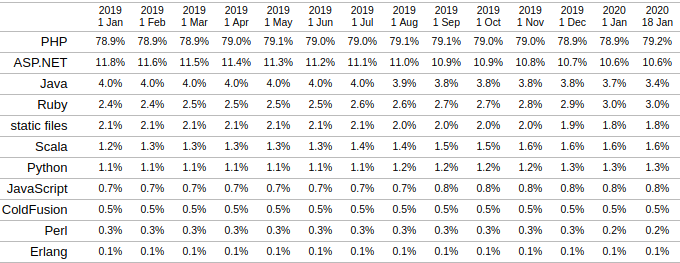
\includegraphics[width=6in]{images/php.png}
    \caption{Przedstawienie użycia języków po stronie serwera na podstawie strony https://w3techs.com/technologies/history\_overview/programming\_language na dzień 12.01.2020  \label{fig:php}}
\end{figure}
        \section{Główne frameworki i biblioteki}
            \subsection{Laravel}
                Jest to najpopularniejszy framework do tworzenia aplikacji internetowych w języku PHP. Zostawił w tyle większość konkurencji, umożliwiając bezkompromisową pracę.  
Jest zbudowany na fundamencie wzorca MVC (ang. Model View Controler).  
Słynie z efektywnej i bardzo eleganckiej składni. Jedną z głównych cech jest czystość kodu i struktury jaką oddaje nam do użytku Laravel.
Pozostałe cechy które warto wymienić to: 

\begin{itemize}
    \item Prosty i szybki system routingu 
    \item Gotowy kontener wstrzykiwania zależności z ogromem funkcji dodatkowych i konfiguracyjnych 
    \item Intuicyjny system ORM dla praktycznie wszystkich najnowszych baz danych 
    \item Precyzyjny system migracji do bazy danych 
    \item Potężny system do obsługi wypełniania bazy danych  
    \item Zadania w tle  
    \item Obsługa i możliwość tworzenia komend 
    \item Mechanizm kolejkowania zadań 
    \item System mailingowy  
    \item System notyfikacji   
    \item Implementacja wielu wzorców projektowych do konkretnych zadań 
    \item System eventowy 
    \item Broadcasting
  \end{itemize}
            \subsection{Vue}
                Jest to biblioteka oparta o język JavaScript. Pozwala na tworzenie złożonych aplikacji webowych składających się z szerokeij listy komponentów.
Oparta jest o architekturę MVVM(ModelView View Model).
Znaczącym plusem jaki posiada ta biblioteka jest jej intuicyjność i łatwość w dostarczeniu gotowych rozwiązań.
Stale zyskuje na populaności poszerzając listę swoich zwolenników (rys. \ref{fig:vue}), oraz ilość biblotek rozszerzającyh.

\begin{figure}[H]
    \centering
    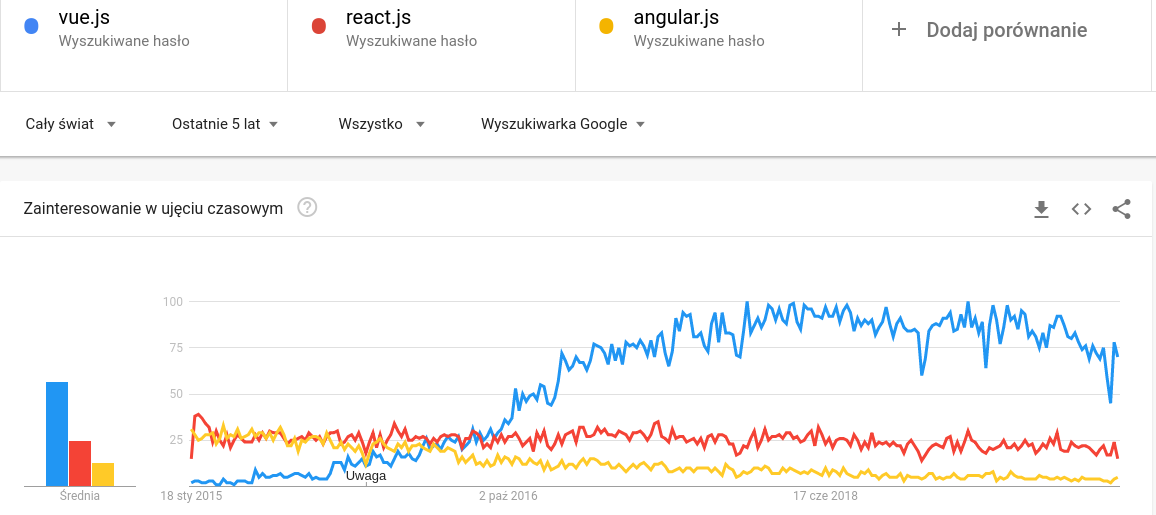
\includegraphics[width=6in]{images/vue.png}
    \caption{Popularność 3 największy frameworków JavaScript na podstawie Google Trends \label{fig:vue}}
\end{figure}
            \subsection{VuetifyJs}
                Vuetify jest frameworkiem na licencji MIT  służacym do budowy interfejsów użytkownika w aplikacjach webowych. Projekt ten jest wspierany przez wolontariuszy i sponsorów z całej społeczności Vue. Posiada spójny cykl aktualizacji, oraz możliwość wykupienia wsparcia dla użytku biznesowego. Co tydzień wypuszczany jest również pakiet poprawek złaszanych przez społeczność

Framework ten obsługuje wszystkie główne przeglądarki. Przeglądarki starsze również będą działać jednak wymagają zastosowania pewnych kroków które można bez problemu znaleźć w dokumentacji.

Vuetify dostarcza również swoje płatne rozwiązania takie jak szablony lub też wcześniej wspomniane wsparcie.

Główną zaletą jest łatwność z jaką tworzy się interfejs przy pomocy gotowych komponenetów. Ich mnogość pozwala na tworzenie dowolnych konfiguracji prze potrzeby tworzenia własnych rozwiązań. Dodatkowo dokumentacja jest przejrzysta i intuicyjna. Zarówno osoba początkująca jak i zaawansowana doceni plusy użytkowania owego frameworku.

Jest to obecnie jedno z lepszych rozwiązań na rynku co poświadcza ilość funkcjonalności dostarczanych przez Vuetify (rys. \ref{fig:vuetifyjs})

\begin{figure}[H]
    \centering
    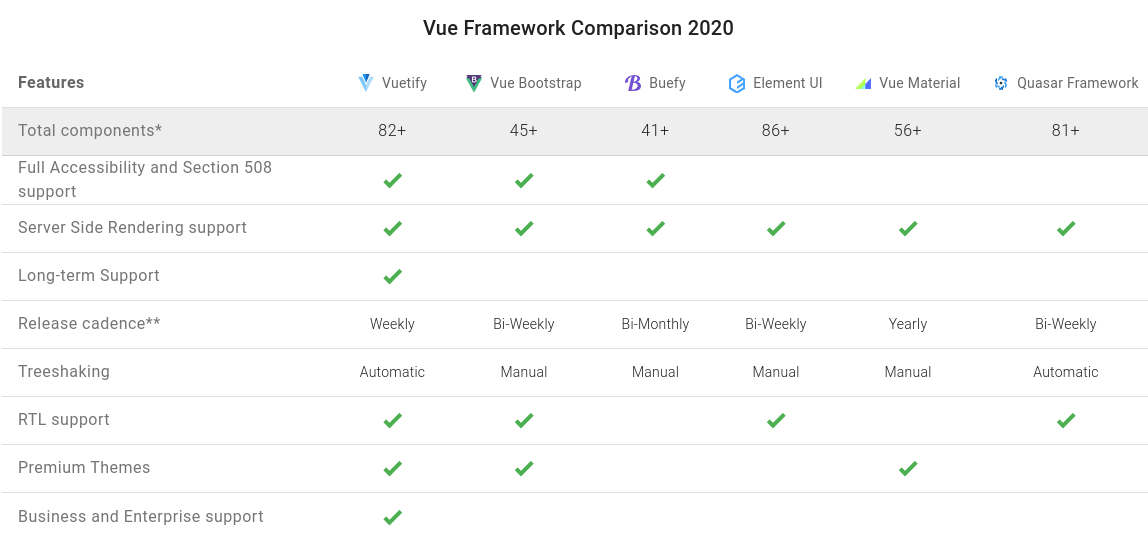
\includegraphics[width=6in]{images/vuetifyjs.png}
    \caption{Porównanie możliwości najbardziej znanych frameworków do Vue \label{fig:vuetifyjs}}
\end{figure}
            \subsection{DOMPDF}
                Jest to darmowa biblioteka która umożliwia konwertowanie języka HTML do plików PDF. Filarem DOMPDF jest jego zgoność ze standardem HTML oraz silnik renderujący utworzony w języku PHP. 
Biblioteka z łatwością otworzy zewnętrzne arkusze stylów, znaczniki inline oraz atrybuty poszczególnych elementów.
Render to pliku PDF możliwy jest dzięki bibliotece PDFLib której posiadanie jest wymogiem do działania.
Główne funkcje jakie dostarcza nam biblioteka to:

\begin{itemize}
    \item obsługa standardu CSS 2.1 oraz częsciowa CSS3
    \item obsługa większości tagów prezentacyjnych ze standardu HTML 4.0
    \item obługa zewnętrznych arkuszy stylów, nawet poprzez dociąganie z serwerów FTP i innych
    \item obsługa rozbudowanych tabel
    \item obsługa większości popularnych formatów zdjęć
    \item brak zewnętrznych zależności
    \item obsługa języka PHP wewnątrz
\end{itemize}
        \section{Narzędzia}
            \subsection{PhpStorm}
                W pełni funkcjonalne, wieloplatformowe PHP IDE zbudowane na bazie IntelliJ IDEA firmy JetBrains. Został on zaprojektowany specjalnie w celu ułatwienia rozwoju aplikacji internetowych napisanych w PHP. Dostarcza wszystkie narzędzia i funkcje dla PHP i obsługuje technologie frontendowe.
Znakomicie radzi sobie z dużymi projektami, podpowiadaniem składni, oraz debugowaniem.
Na dzień dzisiejszy środowisko to jest bezkonkurencyjne. Jest to rozwiązanie płatne jednak z wieloma zniżkami czy też darmowymi wersjami dla studentów.

\begin{figure}[H]
    \centering
    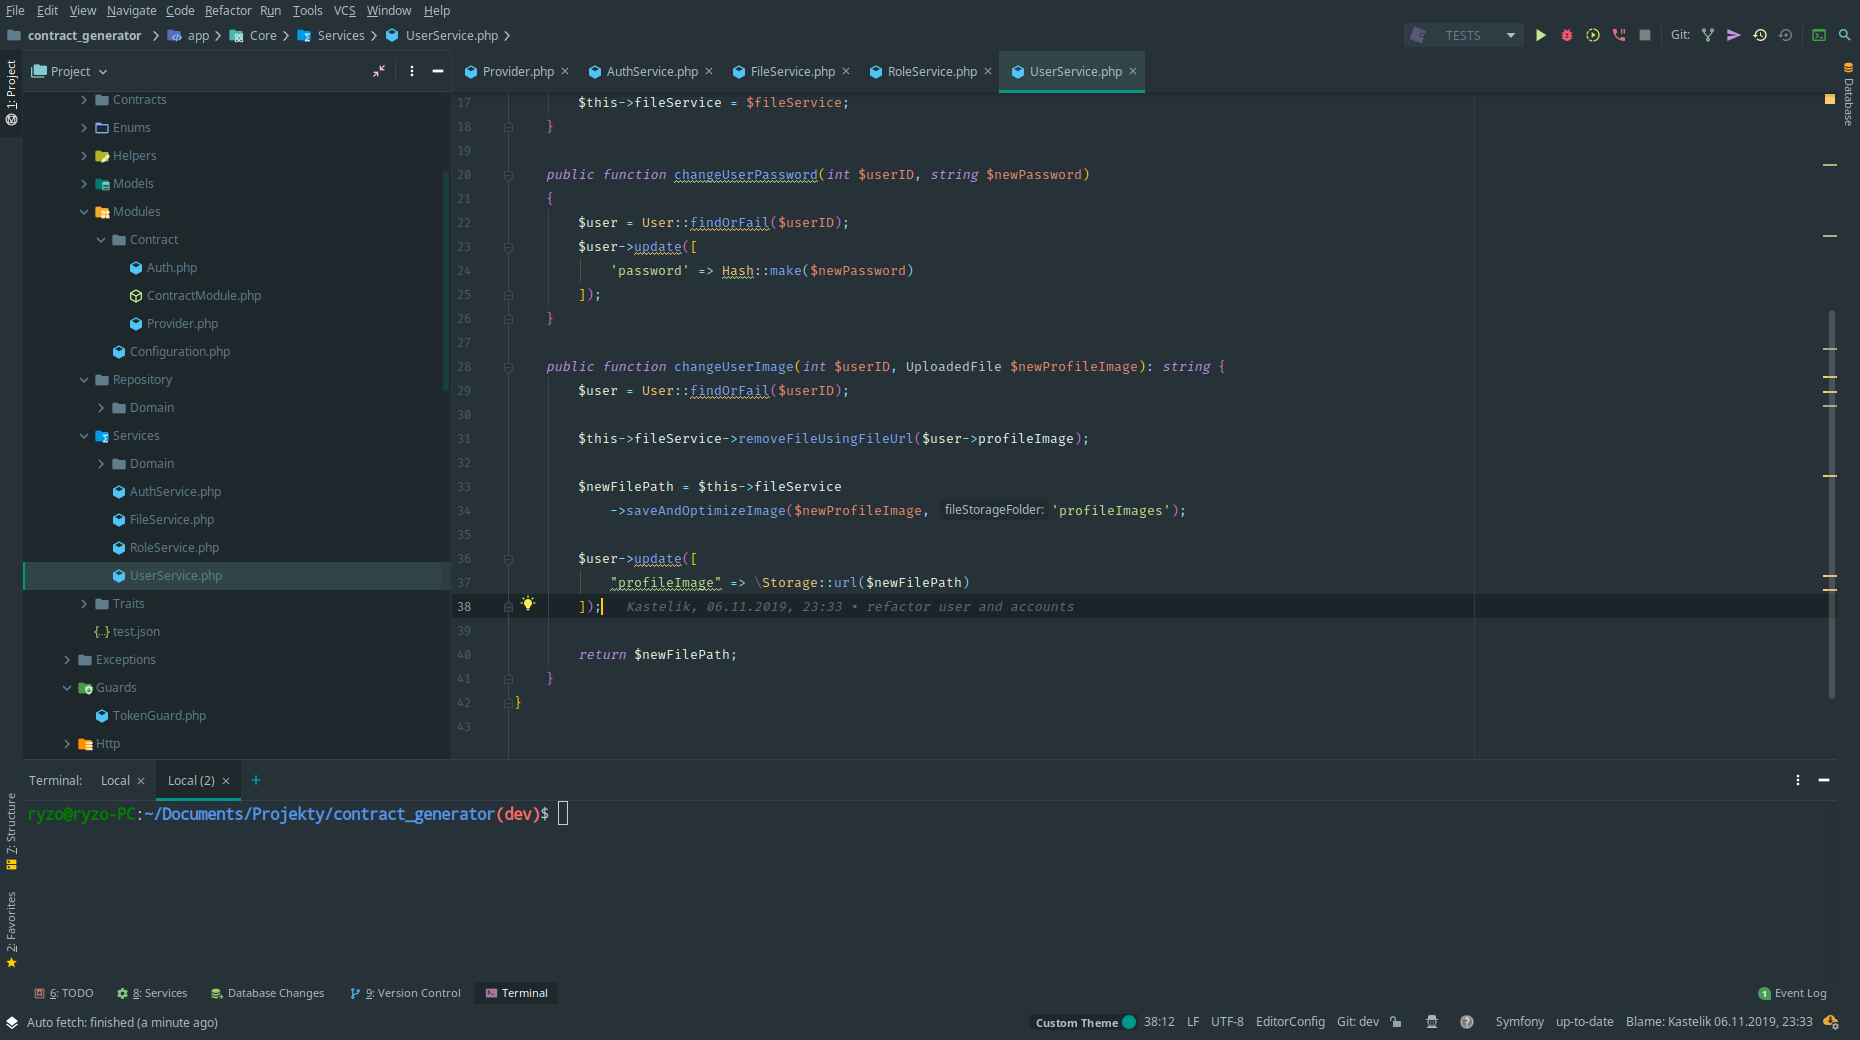
\includegraphics[width=6in]{images/phpstorm.png}
    \caption{Wygląd IDE  w projekcie \label{fig:phpstorm}}
\end{figure}
            \subsection{Git}
                Git jest bardzo popularnym, potężnym i wydajnym systemem kontroli wersji Open Source, który śledzi treści takie jak pliki i katalogi. Jego głównym celem jest zarządzanie projektem lub zestawem plików w miarę ich zmian w czasie.

System kontroli wersji, czyli VCS, jak to się powszechnie określa, jest systemem, który śledzi historię zmian, gdy ludzie i zespoły współpracują ze sobą nad projektami. W miarę jak projekt ewoluuje, zespoły mają możliwość przeprowadzania testów, usuwania błędów i tworzenia nowego kodu z pewnością, że każda wersja może zostać odzyskana w dowolnym momencie.

\begin{figure}[H]
    \centering
    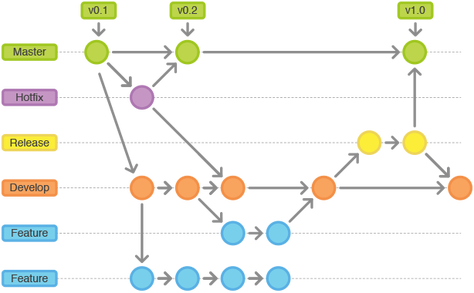
\includegraphics[width=6in]{images/git.png}
    \caption{Przykładowy układ na zasadzie git flow ze strony https://barloblog.wordpress.com \label{fig:git}}
\end{figure}
            \subsection{Docker}
                Docker to narzędzie zaprojektowane w celu ułatwienia tworzenia, wdrażania i uruchamiania aplikacji przy użyciu kontenerów. Kontenery pozwalają programiście na spakowanie aplikacji ze wszystkimi częściami, których potrzebuje, takimi jak biblioteki i inne zależności, i wysłanie jej w jednym pakiecie. W ten sposób, dzięki kontenerowi, deweloper może mieć pewność, że aplikacja będzie działać na każdej innej maszynie, bez względu na wszelkie niestandardowe ustawienia, które maszyna może mieć, a które mogą się różnić od tych, które są używane do pisania i testowania kodu, a także od serwera produkcyjnego.

W pewnym sensie, Docker jest trochę jak wirtualna maszyna. Ale w przeciwieństwie do maszyny wirtualnej, zamiast tworzyć cały wirtualny system operacyjny, Docker pozwala aplikacjom korzystać z tego samego jądra Linuksa co system, na którym są uruchomione i wymaga tylko dostarczenia aplikacji z rzeczami, które nie są jeszcze uruchomione na komputerze hosta. Daje to znaczący wzrost wydajności i zmniejsza rozmiar aplikacji.
        \section{Usługi}
            \subsection{VPS DigitalOcean}
                

DigitalOcean jest znanym dostawcą chmury obliczeniowej który oferuje infrastrukturę zgodną z zasadą IaaS (ang. Infrastructure as a Service) dla twórców oprogramowania. Jest bardzo popularny i znakomicie konkuruje z AWS (ang. Amazon Web Services) czy też Google Compute Engine.

W celu uruchomienia środowiska programiści uruchamiają instancję prywatnej maszyny wirtualnej (VM) która w DigitalOcean nosi nazwę droplet(kropelka). Użytkownik może wybrać wielkość kropelki, region geograficzny i centrum danych w którym będziue ona działać oraz system operacyjny z rodziny Linux.
Można jednocześnie użyć swoich obrazów do postawienia gotowego środowiska uruchomieniowego.

Aktualnie dostawca oferuje czternaście rozmiarów kropli. Najmniejszy rozmiar zaczyna się od 1GB pamięci RAM z 1 procesorem i 25GB pamięci SSD, taki układ to koszt 5\$ miesięcznie ( rys. \ref{fig:digitalocean}). Wraz ze wzrostem specyfikacji rośnie również cena, aby maksymalnie osiągnąć 960\$ za 192GB pamięci RAM z 32 procesorami i 12TB pamięci SSD.

Deweloperzy używają systemu DigitalOcean do zarządzania i monitorowania kropli za pomocą panelu sterowania i API open source. Panel kontrolny umożliwia deweloperom skalowanie i przebudowę kropli na podstawie zmian w obciążeniu pracą oraz wykonywanie kopii zapasowych i przekierowywanie ruchu sieciowego pomiędzy kropelkami.

DigitalOcean został założony w 2011 roku przez Bena Ureckiego, Moiseya Ureckiego, Mitcha Wainera, Jeffa Carra i Aleca Hartmana. Siedziba firmy znajduje się w Nowym Jorku.


\begin{figure}[H]
    \centering
    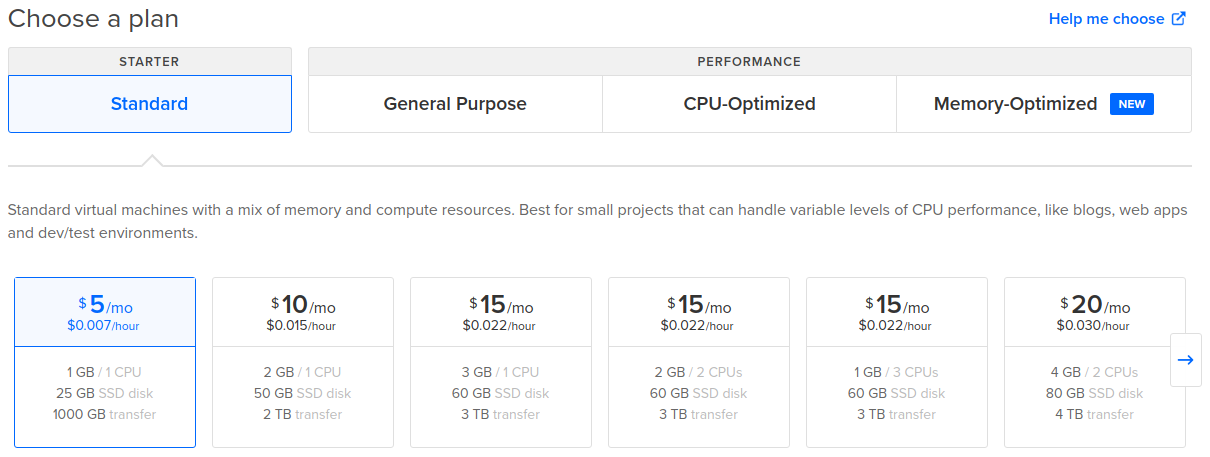
\includegraphics[width=6in]{images/digitalocean.png}
    \caption{Wybór mozliwych konfiguracji na stronie https://cloud.digitalocean.com \label{fig:digitalocean}}
\end{figure}
            \subsection{Domena generatorumowy.pl}
                W celu utworzenia projektu koniecznym było wystawienie go dla osób trzecich, aby umozliwić testowanie przez osoby niezwiązane z pracą.
Domena jest to podstawowy inedytifkator tożsamości w internecie. Jest to element adresu internetowego aplikacji webowych.
Każdy może zakupić wolną domenę dla swoich celów. Należy w tym celu znaleźć odpowiadającego nam dostawcę i wykupić domenę o podanej nazwie.
Po tym procesie możemy bez problemu przekierować ją na żądany hosting lub też maszynę serwerową (rys. \ref{fig:domain}).

\begin{figure}[!ht]
    \centering
    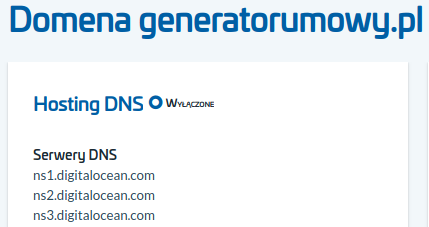
\includegraphics[width=5in]{images/domain.png}
    \caption{Przykładowa konfiguracja u dostawy az.pl \label{fig:domain}}
\end{figure}
            \subsection{SSL}
                Certyfikaty SSL to niewielkie pliki danych, które w sposób cyfrowy wiążą klucz kryptograficzny z danymi organizacji. Po zainstalowaniu na serwerze WWW, aktywuje on kłódkę i protokół https oraz umożliwia bezpieczne połączenia z serwera WWW do przeglądarki. Zazwyczaj SSL jest używany do zabezpieczania transakcji kartami kredytowymi, przesyłania danych i logowania, a ostatnio staje się normą przy zabezpieczaniu przeglądania stron serwisów społecznościowych.
Do naszych celów certyfikat został wygenerowany dzięki darmowemu urządowi certyfikacji Let's Encrypt (rys. \ref{fig:ssl}).

\begin{figure}[H]
    \centering
    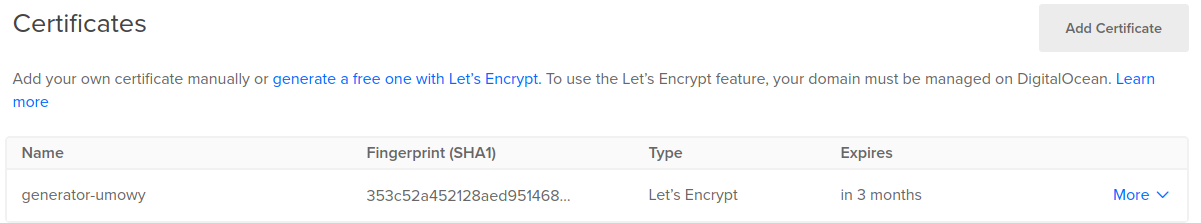
\includegraphics[width=6in]{images/ssl.png}
    \caption{Przykład dodania certyfikatu na stronie https://cloud.digitalocean.com \label{fig:ssl}}
\end{figure}
            \subsection{Forge}
                Laravel Forge jest narzędziem do wdrażania i konfigurowania aplikacji internetowych. Został opracowany przez twórców szkieletu Laravela, ale może być użyty do zautomatyzowania wdrożenia dowolnej aplikacji internetowej, która korzysta z serwera PHP.

Tworzenie w pełni funkcjonalnego serwera WWW zazwyczaj wymaga instalacji wielu komponentów, takich jak NGINX, MySQL i PHP. Laravel Forge automatyzuje wszystkie niezbędne kroki instalacji i konfiguracji, co pozwala na szybkie uruchomienie witryny.

Po utworzeniu serwera, wdrażanie aktualizacji staje przejrzyste i bezbolesne. Ponadto, można łatwo zarządzać konfiguracją swojej strony internetowej za pomocą interfejsu WWW. Wreszcie, Forge automatycznie udostępnia zaawansowane funkcje bezpieczeństwa, takie jak darmowe certyfikaty SSL (poprzez Let's Encrypt) i automatyczną konfigurację firewalla.

\begin{figure}[H]
    \centering
    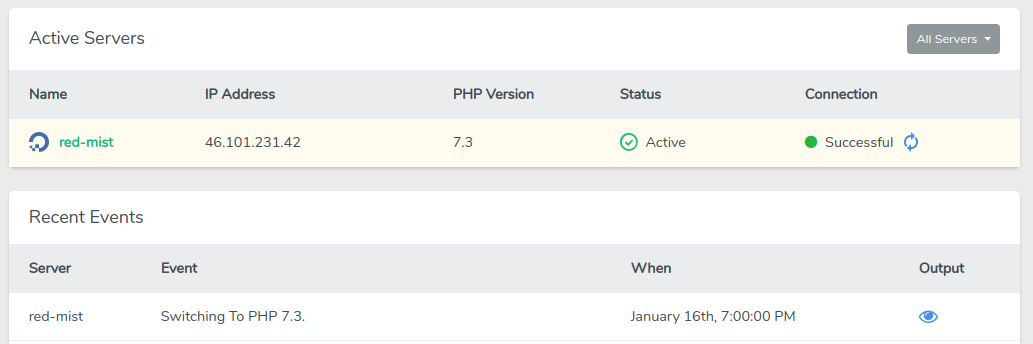
\includegraphics[width=6in]{images/forge.png}
    \caption{Przykład dodania certyfikatu na stronie https://cloud.digitalocean.com \label{fig:forge}}
\end{figure}
            \subsection{Jenkins}
                Jenkins jest narzędziem automatyki open source napisanym w języku Java z wtyczkami zbudowanymi dla celów ciągłej integracji (ang. Continous Integration). Jenkins jest używany do budowania i testowania projektów oprogramowania w sposób ciągły, ułatwiając programistom integrowanie zmian w projekcie i ułatwiając użytkownikom uzyskanie nowej konstrukcji. Pozwala również na ciągłe dostarczanie oprogramowania poprzez integrację z dużą liczbą technologii testowych i wdrożeniowych.

Dzięki Jenkinsowi, organizacje mogą przyspieszyć proces tworzenia oprogramowania poprzez automatyzację. Jenkins integruje wszelkiego rodzaju procesy cyklu życia oprogramowania, w tym tworzenie, dokumentowanie, testowanie, pakowanie, etapowanie, wdrażanie, analizę statyczną i wiele innych.

W naszym przypadku Jenkins odpowiada za proces testowania oraz wdrożeniowy. Udane testy wysyłaja zapytanie o chęć wdrożenia najnowszej zmiany. Po pozytywnym rozpatrzeniu wysyłane jest odpowiednie zdarzenie do wcześniej przedstawionej platformy forge która zajmuje się wgraniem na serwer najnowszej wersji oprogramowania (rys. \ref{fig:jenkins}).

\begin{figure}[H]
    \centering
    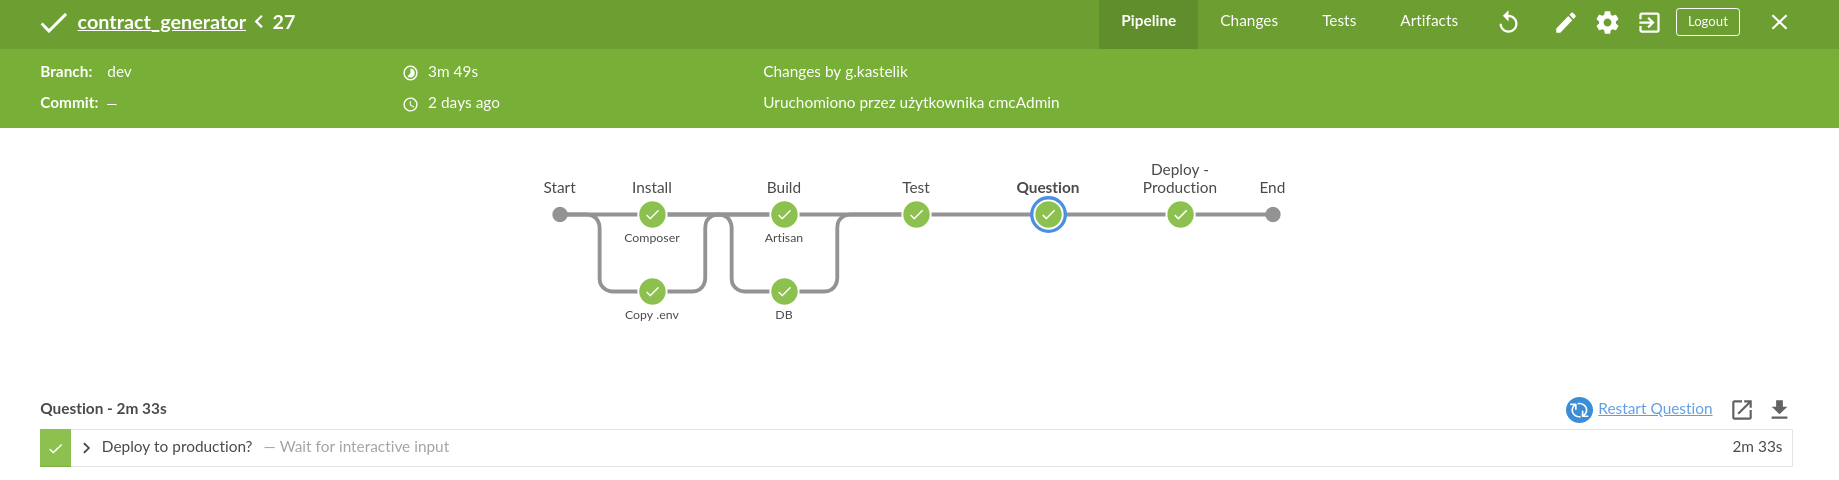
\includegraphics[width=6in]{images/jenkins.png}
    \caption{Proces testowania i wdrażania aplikacji \label{fig:jenkins}}
\end{figure}

\begin{figure}[H]
    \centering
    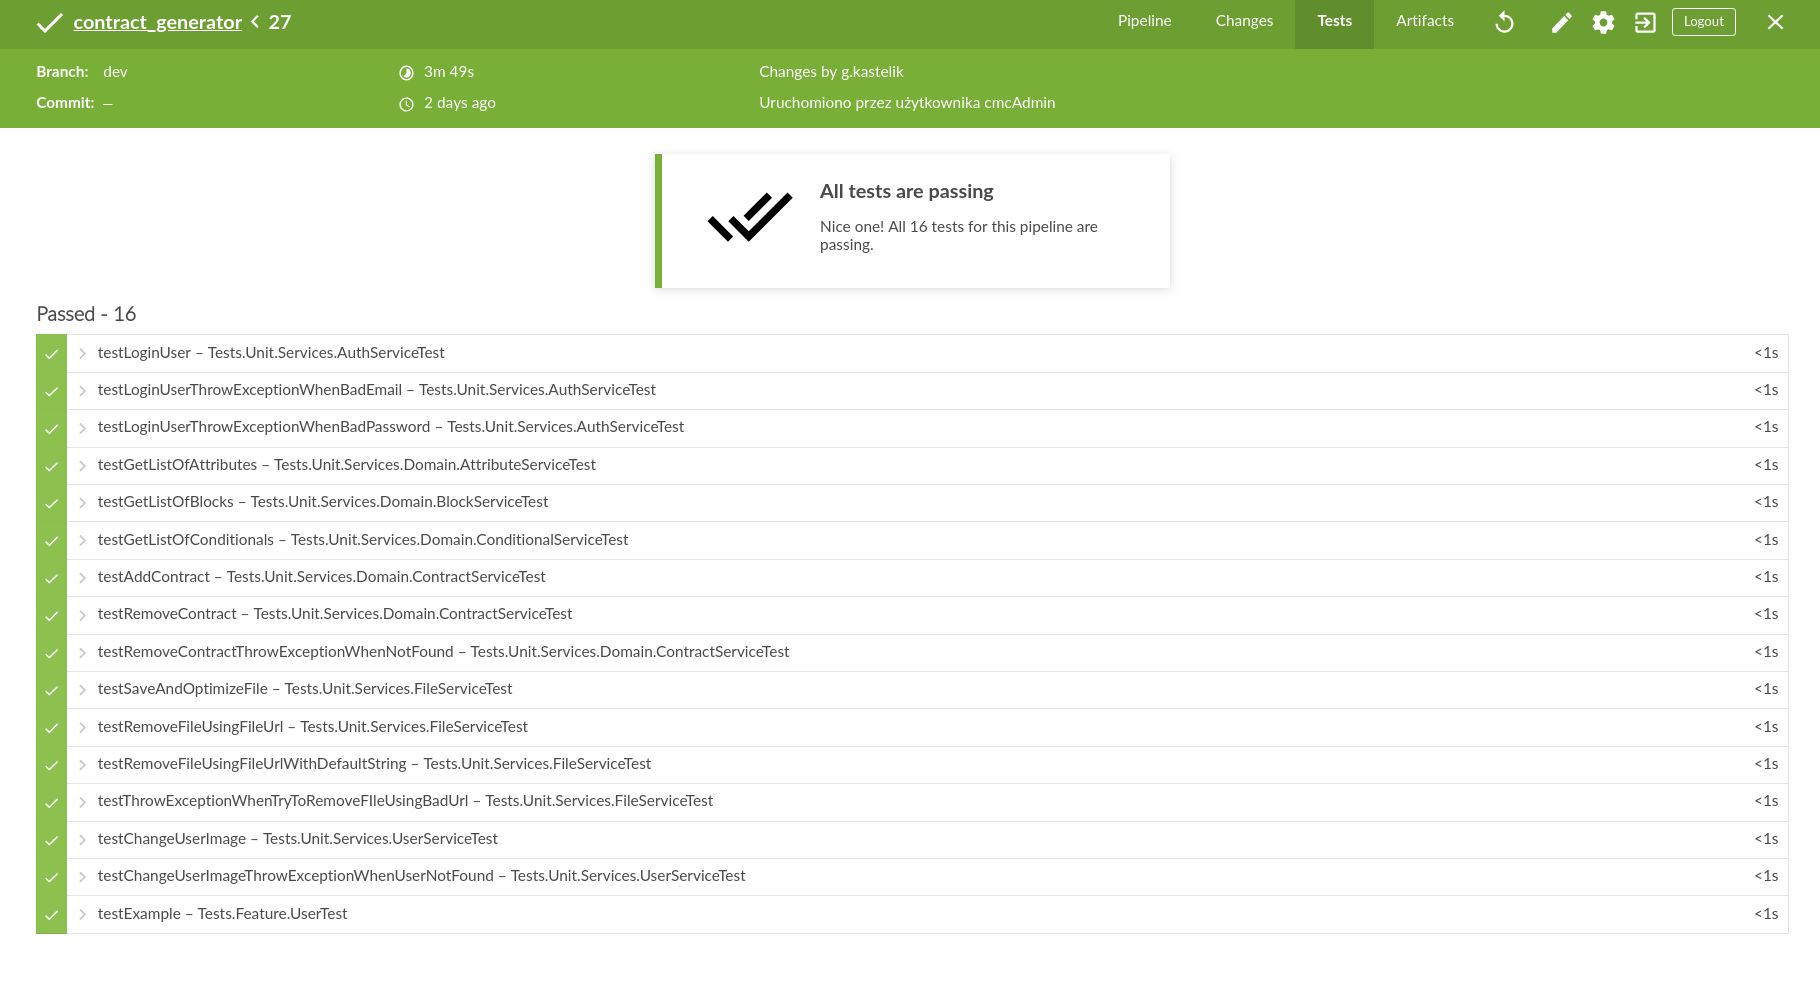
\includegraphics[width=6in]{images/jenkins-test.png}
    \caption{Raport na temat testów przeprowadzonych na aplikacji \label{fig:jenkins-test}}
\end{figure}


    \chapter{Projekt systemu tworzenia umów}
         \section{Opis działania systemu}
         \section{Schemat bazodanowy}
    \chapter{Opis platformy implementującej system}
        \section{Platforma}
            \subsection{Implementacja}
            \subsection{Instrukcja użytkowania}
        \section{API}
            \subsection{Implementacja}
            \subsection{Instrukcja użytkowania}
            \subsection{Testy}
    \chapter{Podsumowanie oraz wnioski}
    \listoffigures
    \begin{thebibliography}{99}
    \bibitem{enc-zarzadzania} Strona internetowa https://mfiles.pl/pl/index.php/Umowa - Encyklopedia Zarządzania - Dostępna na dzień 12.01.2020 
    \bibitem{API} Strona internetowa https://marketingwsieci.pl/slownik-e-marketingu/api-application-programming-interface/ - Blog firmy MAYKO - Dostępna na dzień 12.01.2020 
\end{thebibliography}
\end{document}